\chapter{MARCO TEÓRICO}
\label{chap:marco-teorico}

Este capítulo establece los fundamentos teóricos y tecnológicos que sustentan el desarrollo de ``TecnoTime''. Se abordan los paradigmas de ingeniería de software móvil moderna, la arquitectura de software escalable, los algoritmos de optimización para la generación de horarios y la integración de inteligencia artificial en el borde (Edge AI). Cada sección vincula los conceptos académicos con las tecnologías específicas implementadas en la solución.

\section{Ingeniería de Software para Dispositivos Móviles}
\label{sec:ingenieria-movil}

El desarrollo de aplicaciones móviles ha transitado desde enfoques imperativos hacia paradigmas declarativos y reactivos, priorizando la eficiencia en el manejo de recursos limitados y la experiencia de usuario fluida.

\subsection{Arquitectura de Plataforma Android}
Android es un sistema operativo basado en el núcleo Linux, diseñado para dispositivos con pantalla táctil. Su arquitectura se divide en capas: el kernel de Linux, la capa de abstracción de hardware (HAL), el tiempo de ejecución de Android (ART) y el marco de trabajo de aplicaciones (Application Framework) \cite{android_arch}.

El desarrollo nativo, utilizando el Android SDK (Software Development Kit), permite un acceso directo a las APIs del sistema y un rendimiento superior en comparación con soluciones híbridas, especialmente en tareas intensivas como la inferencia de modelos de IA \cite{android_programming}. En este proyecto se utiliza Kotlin, un lenguaje moderno y estáticamente tipado que interoperan completamente con Java, aprovechando características como Coroutines y Flow para la gestión eficiente de la concurrencia asíncrona.

\subsection{Paradigma de Interfaz Declarativa (Jetpack Compose)}
Tradicionalmente, las interfaces en Android se construían manipulando un árbol de vistas XML (enfoque imperativo). La tendencia actual en la industria, respaldada por estudios comparativos de rendimiento y mantenibilidad \cite{singh2025comparative, jain2023compose}, es el uso de marcos de trabajo declarativos.

El Cuadro \ref{tab:imperative_vs_declarative} resume las diferencias clave entre ambos paradigmas.

\begin{table}[h!]
    \centering
    \caption{Comparación entre UI Imperativa y Declarativa}
    \label{tab:imperative_vs_declarative}
    \begin{tabular}{|p{6cm}|p{6cm}|}
        \hline
        \textbf{Enfoque Imperativo (XML)} & \textbf{Enfoque Declarativo (Compose)} \\
        \hline
        Se manipula manualmente el árbol de vistas (DOM/Views). & La UI se describe como una función del estado. \\
        \hline
        El estado de la UI y el estado de la app pueden desincronizarse. & El estado es la única fuente de verdad. \\
        \hline
        Mucho código repetitivo (boilerplate). & Código más conciso y legible. \\
        \hline
    \end{tabular}
    \vspace{0.2cm}
    \\
    \small{Fuente: Basado en Singh et al. (2025) \cite{singh2025comparative}}
\end{table}

``TecnoTime'' adopta Jetpack Compose, el kit de herramientas moderno de Android. En este paradigma, la interfaz se describe como una función del estado actual de la aplicación. Cuando el estado cambia, el marco de trabajo ejecuta un proceso de Recomposición, actualizando inteligentemente solo los componentes que dependen de los datos modificados, lo que reduce la complejidad de sincronización manual entre la vista y el modelo \cite{gupta2022modern}.

\subsection{Ciclo de Vida y Gestión de Estado (UDF)}
La gestión de estado es crítica en aplicaciones reactivas para garantizar la consistencia de los datos mostrados. Se utiliza el patrón Unidirectional Data Flow (UDF), donde el estado fluye en una sola dirección (de la lógica a la UI) y los eventos fluyen en sentido contrario (de la UI a la lógica).

Para implementar esto, se emplean flujos reactivos mediante StateFlow de la librería Kotlin Coroutines. StateFlow es un flujo observable que emite actualizaciones de estado inmutables a la interfaz de usuario, asegurando que la UI siempre refleje el último estado válido producido por la capa de lógica de negocio \cite{reactive_kotlin}.

\section{Arquitectura de Software}
\label{sec:arquitectura-software}

Para garantizar la mantenibilidad, testabilidad y escalabilidad del proyecto, se siguen principios de diseño robustos y patrones arquitectónicos estandarizados en la industria del software.

\subsection{Clean Architecture y Regla de Dependencia}
El proyecto implementa Clean Architecture, propuesta por Robert C. Martin \cite{martin2017-cleanarch}. Esta arquitectura estructura el código en capas concéntricas con responsabilidades claras, como se ilustra en la Figura \ref{fig:clean_architecture}.

\begin{figure}[h!]
    \centering
    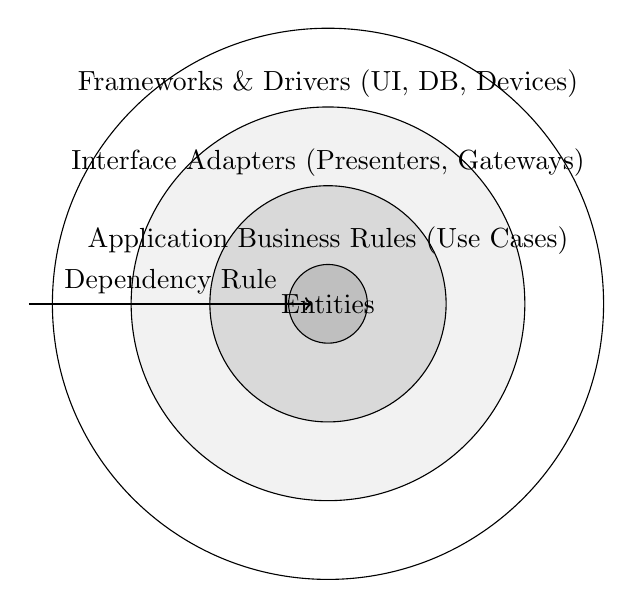
\begin{tikzpicture}
        \draw[fill=white] (0,0) circle (3.5cm);
        \node at (0, 2.8) {Frameworks \& Drivers (UI, DB, Devices)};
        
        \draw[fill=gray!10] (0,0) circle (2.5cm);
        \node at (0, 1.8) {Interface Adapters (Presenters, Gateways)};
        
        \draw[fill=gray!30] (0,0) circle (1.5cm);
        \node at (0, 0.8) {Application Business Rules (Use Cases)};
        
        \draw[fill=gray!50] (0,0) circle (0.5cm);
        \node at (0, 0) {Entities};
        
        % Dependency Arrow
        \draw[->, thick] (-3.8, 0) -- (-0.2, 0);
        \node[anchor=south] at (-2, 0) {Dependency Rule};
    \end{tikzpicture}
    \caption{Diagrama conceptual de Clean Architecture}
    \label{fig:clean_architecture}
    \small{Fuente: Basado en Martin (2017) \cite{martin2017-cleanarch}}
\end{figure}

Las capas principales son:
\begin{itemize}
    \item Capa de Dominio (Domain): Contiene la lógica de negocio pura (Entidades y Casos de Uso). Es la capa más interna y no tiene dependencias de frameworks externos.
    \item Capa de Datos (Data): Implementa las interfaces definidas por el dominio y gestiona las fuentes de datos (base de datos local, red).
    \item Capa de Presentación (Presentation): Contiene la UI y los adaptadores de vista.
\end{itemize}
La Regla de Dependencia establece que las dependencias de código fuente solo pueden apuntar hacia adentro; el dominio no conoce detalles de la base de datos ni de la interfaz de usuario, lo que permite cambiar estas capas externas sin afectar la lógica central.

\subsection{Patrón Model-View-ViewModel (MVVM)}
Se utiliza el patrón MVVM para separar la lógica de presentación de la interfaz de usuario. La Figura \ref{fig:mvvm_pattern} muestra la interacción entre sus componentes.

\begin{figure}[h!]
    \centering
    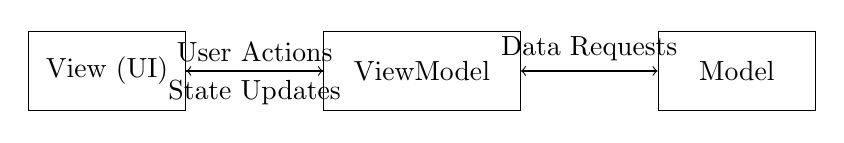
\begin{tikzpicture}[node distance=2cm, auto]
        \node (view) [draw, rectangle, minimum width=2cm, minimum height=1cm] {View (UI)};
        \node (viewmodel) [draw, rectangle, right of=view, node distance=4cm, minimum width=2.5cm, minimum height=1cm] {ViewModel};
        \node (model) [draw, rectangle, right of=viewmodel, node distance=4cm, minimum width=2cm, minimum height=1cm] {Model};

        \draw[->] (view) -- node {User Actions} (viewmodel);
        \draw[->] (viewmodel) -- node {State Updates} (view);
        \draw[<->] (viewmodel) -- node {Data Requests} (model);
    \end{tikzpicture}
    \caption{Patrón Model-View-ViewModel (MVVM)}
    \label{fig:mvvm_pattern}
    \small{Fuente: Basado en Google Developers \cite{android_arch}}
\end{figure}

\begin{itemize}
    \item Model: Representa los datos y la lógica de negocio (Capa de Dominio).
    \item View: La interfaz de usuario (Compose) que observa el estado.
    \item ViewModel: Actúa como intermediario, exponiendo el estado de la UI y procesando las interacciones del usuario. En Android, los ViewModels están diseñados para sobrevivir a cambios de configuración, como la rotación de pantalla \cite{pro_android_kotlin}.
\end{itemize}

\subsection{Inyección de Dependencias (Hilt)}
La Inyección de Dependencias (DI) es un patrón de diseño donde los objetos reciben sus dependencias desde fuera en lugar de crearlas ellos mismos, promoviendo la Inversión de Control (IoC) \cite{dependency_injection_principles}.

Se utiliza Hilt, la solución estándar de Google para DI en Android basada en Dagger. Hilt reduce el código repetitivo y gestiona el ciclo de vida de los componentes, facilitando la modularidad y permitiendo el intercambio de implementaciones (por ejemplo, inyectar repositorios simulados durante las pruebas automatizadas).

\section{Algoritmia de Planificación (Timetabling)}
\label{sec:algoritmia}

El núcleo funcional de la aplicación aborda el problema de generación de horarios académicos, conocido formalmente en la literatura como University Course Timetabling Problem (UCTP).

\subsection{Problema de Satisfacción de Restricciones (CSP)}
El UCTP se modela matemáticamente como un Problema de Satisfacción de Restricciones (CSP), definido por Russell y Norvig \cite{russell2021ai} como una terna $(X, D, C)$:
\begin{itemize}
    \item $X$: Un conjunto de variables (las asignaturas a inscribir).
    \item $D$: Un conjunto de dominios (los grupos disponibles para cada asignatura).
    \item $C$: Un conjunto de restricciones que especifican combinaciones permitidas de valores.
\end{itemize}
Las restricciones se clasifican en Duras (Hard), que deben cumplirse obligatoriamente (ej. no solapamiento de horarios), y Blandas (Soft), que expresan preferencias deseables pero no obligatorias (ej. minimizar huecos libres).

\subsection{Algoritmos de Búsqueda: Backtracking}
Para resolver el CSP, se implementa el algoritmo de Backtracking (Vuelta Atrás). Este es un algoritmo de búsqueda en profundidad que construye candidatos a solución de manera incremental. Si se añade una asignación que viola una restricción dura, el algoritmo ``retrocede'' al paso anterior y prueba con el siguiente valor del dominio, descartando esa rama del árbol de búsqueda \cite{cormen_algorithms}.

\subsection{Heurísticas de Poda y Optimización}
Dado que el espacio de búsqueda puede crecer exponencialmente, se aplican heurísticas para mejorar la eficiencia:
\begin{itemize}
    \item Poda (Pruning): Se descartan tempranamente las ramas que no pueden llevar a una solución válida (ej. si una materia obligatoria se queda sin cupos válidos).
    \item Ordenamiento de Variables (Fail-First): Se intentan asignar primero las variables más restrictivas para detectar conflictos lo antes posible \cite{automated_timetabling}.
    \item Función Objetivo: Las soluciones válidas encontradas se evalúan mediante una función de puntuación ponderada que penaliza los huecos y bonifica la asignación de docentes preferidos.
\end{itemize}

\section{Inteligencia Artificial en Dispositivos Móviles (Edge AI)}
\label{sec:edge-ai}

``TecnoTime'' integra capacidades de inteligencia artificial generativa ejecutándose directamente en el dispositivo móvil, un paradigma conocido como Edge AI.

\subsection{Inferencia Local vs. Inferencia en la Nube}
A diferencia de la IA en la nube, la Edge AI procesa los datos localmente en el dispositivo del usuario. El Cuadro \ref{tab:edge_vs_cloud} compara ambos enfoques.

\begin{table}[h!]
    \centering
    \caption{Comparación entre Edge AI y Cloud AI}
    \label{tab:edge_vs_cloud}
    \begin{tabular}{|p{5cm}|p{5cm}|}
        \hline
        \textbf{Edge AI (Local)} & \textbf{Cloud AI (Nube)} \\
        \hline
        Procesamiento en el dispositivo. & Procesamiento en servidores remotos. \\
        \hline
        Privacidad total (datos no salen). & Riesgo de privacidad al enviar datos. \\
        \hline
        Latencia baja (tiempo real). & Latencia depende de la red. \\
        \hline
        Funciona sin internet (Offline). & Requiere conexión constante. \\
        \hline
    \end{tabular}
    \vspace{0.2cm}
    \\
    \small{Fuente: Basado en Pothineni (2024) \cite{pothineni2024offline} y Shi et al. (2023) \cite{edge_ai_arxiv}}
\end{table}

En la implementación, se utiliza la librería llama.cpp a través de JNI (Java Native Interface) para ejecutar la inferencia de modelos de lenguaje de manera eficiente en la CPU del dispositivo Android.

\subsection{Modelos de Lenguaje (LLMs) y Cuantización}
Para viabilizar la ejecución de Large Language Models (LLMs) en dispositivos con recursos limitados (memoria y batería), se utiliza la técnica de Cuantización. Este proceso reduce la precisión de los pesos del modelo (por ejemplo, de punto flotante de 16 bits a enteros de 4 bits), disminuyendo drásticamente el tamaño del modelo y el consumo de memoria con una pérdida mínima de precisión \cite{quantization_papers}. El formato de archivo utilizado es GGUF, optimizado para inferencia rápida en CPU.

\section{Gestión y Persistencia de Datos}
\label{sec:persistencia}

La aplicación sigue una filosofía Offline-First, garantizando que la funcionalidad principal esté disponible sin conexión a internet, un requisito crítico en entornos con conectividad intermitente \cite{guda2025offline}.

\subsection{Bases de Datos Relacionales Embebidas (Room)}
Para la persistencia local se utiliza SQLite, un motor de base de datos relacional ligero embebido en Android. El acceso se gestiona a través de la librería Room, que proporciona una capa de abstracción orientada a objetos sobre SQLite, permitiendo definir Entidades y DAOs con verificación de consultas SQL en tiempo de compilación \cite{database_concepts}.

\subsection{Estrategias de Sincronización y Offline-First}
\begin{figure}[h!]
    \centering
    \includegraphics[width=0.8\textwidth]{images/offline_architecture_couchbase.png}
    \caption{Arquitectura típica de una aplicación Offline-First}
    \label{fig:offline_architecture}
    \small{Fuente: Couchbase Inc. (2023) \cite{couchbase_offlinefirst}}
\end{figure}

La arquitectura adopta el principio de Single Source of Truth (SSOT). La interfaz de usuario siempre observa y muestra los datos de la base de datos local. Las operaciones de red para actualizar los horarios se ejecutan en segundo plano utilizando WorkManager, un planificador de tareas diferibles y garantizadas. Cuando la sincronización completa, se actualiza la base de datos local, y Room notifica automáticamente a la UI para que refleje los cambios, desacoplando así la experiencia de usuario de la latencia de la red.
